
\begin{figure}
	\centering
	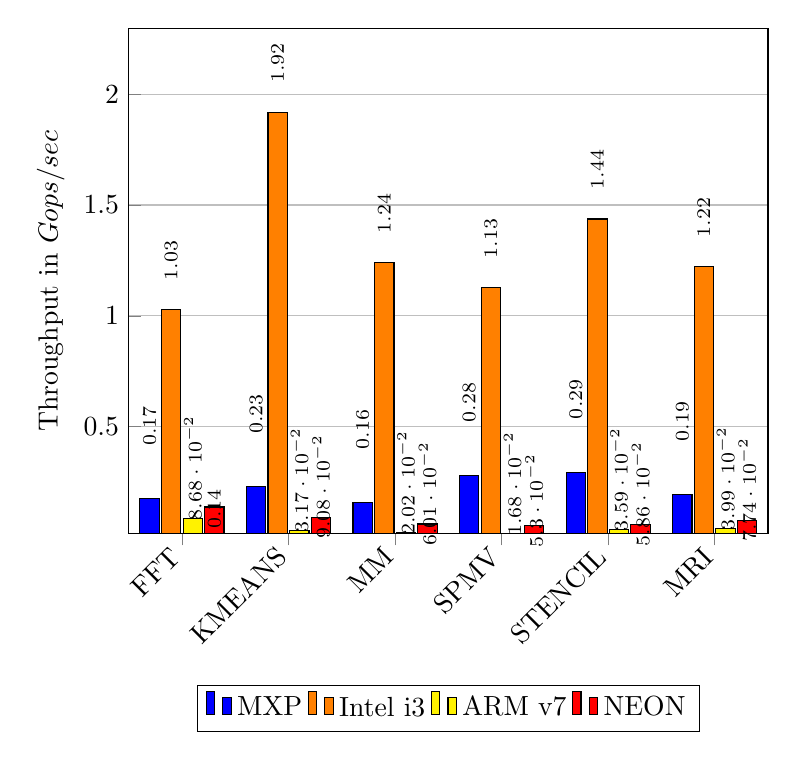
\begin{tikzpicture}
	\begin{axis}[
	width  = 0.8*\textwidth,
	height = 8cm,
	xtick pos=left,
	ytick pos=left,
%	major x tick style = transparent,
	x tick label style={rotate=45, anchor=east, align=right,text width=2cm},
	bar width=7pt,
	ymajorgrids = true,
	ylabel = {Throughput in $Gops/sec$},
	symbolic x coords={FFT,KMEANS,MM,SPMV,STENCIL,MRI},
	xtick = data,
	nodes near coords,
	ybar,
	every node near coord/.append style={rotate=90, anchor=west,font=\scriptsize, xshift=0.25cm},
	scaled y ticks = false,
	enlarge y limits={upper,value=0.2},
%	enlarge x limits=0.25,
	ybar=2*\pgflinewidth,
	legend cell align=left,
	legend style={
	at={(.5,-0.3)},
	anchor=north,
	legend columns=-1
	column sep=0.5ex
}
	]
	\addplot[draw=black,fill=blue,every node near coord/.append style={xshift=0.3cm}]
	coordinates {(FFT,0.174) (KMEANS,0.2285) (MM,0.1567) (SPMV,0.2798) (STENCIL,0.2945) (MRI,0.194)};
	
	\addplot[draw=black,fill=orange]
	coordinates  {(FFT,1.0283) (KMEANS,1.918) (MM,1.24) (SPMV,1.126) (STENCIL,1.437) (MRI,1.2211)};
	
	\addplot[draw=black,fill=yellow,every node near coord/.append style={xshift=-0.4cm}]
	coordinates  {(FFT, 0.08677) (KMEANS,0.03174) (MM,0.02015) (SPMV,0.01680) (STENCIL,0.03589) (MRI,0.0399)};
	
	\addplot[draw=black,fill=red,every node near coord/.append style={xshift=-0.65cm}]
	coordinates {(FFT, 0.13705) (KMEANS,0.0908) (MM,0.06009) (SPMV,0.053) (STENCIL,0.0586) (MRI,0.07735)};
	
	\legend{MXP,Intel i3,ARM v7,NEON}
	\end{axis}
	\end{tikzpicture}
	\caption{Word(32-bits) level throughput(Gops/sec) for compute Kernels}
	\label{kernel:3}
\end{figure}